\section{Étude expérimentale}
Cette section présente les différents outils utilisés à l'aboutissement de l'application réalisée ainsi que l'architecture de l'application développée.
A partir de l'application développée nous réalisons une étude expérimentale d'un exemple issu de la vie courante, ensuite nous interprétons les résultats expérimentaux obtenus par la méthode de redistribution proposée dans ce chapitre.

\subsection{Outils de développement}
Pour la mise en œuvre d’une application de distribution de l'espace d'états et de la vérification formelle, la capacité à monter en charge s’envisage pour pouvoir évoluer de façon fluide en fonction de l'augmentation de la demande des ressources afin qu'une expérimentation soit menée dans les meilleures conditions. Dans ce qui suit nous pressentons les outils nécessaires pour le développement de ce type d'application. \newpage

\subsubsection*{Langage de programmation Java}
\begin{wrapfigure}{r}{0.2\textwidth}
	\vspace{-60pt}
	\begin{center}
		
\includegraphics[width=0.1\textwidth]{img/java}
	\end{center} 
	\vspace{-20pt}
	\vspace{-10pt} 
\end{wrapfigure}
Java est un langage de programmation moderne orientée objet développé par Sun Microsystems (aujourd'hui racheté par Oracle) \citep{java}. Le langage Java permet la programmation parallèle, le développement des applications reparties, l'accès à des bases de données, l'accès à des traitements en d'autres langages. Ainsi, les applications développées sous le langage  Java sont portables sur plusieurs systèmes d’exploitation tels que Unix, Windows, Mac OS ou GNU/Linux. Par contre elles sont plus lourdes à l'exécution (en mémoire et en temps processeur) à cause de sa machine virtuelle.
\subsubsection*{La plateforme JADE}
\begin{wrapfigure}{r}{0.2\textwidth}
	\vspace{-60pt}
	\begin{center}
		
\includegraphics[width=0.3\textwidth]{img/jade}
	\end{center} 
	\vspace{-20pt}
	\vspace{-10pt} 
\end{wrapfigure}
JADE (Java Agent Development Framework) est une plateforme de programmation multi-agent implémentée en Java \citep{jade}. Elle est open-source et distribuée par Telecom Italia sous la licence LGPL. La plateforme héberge un ensemble d’agents, identifiés de manière unique, pouvant communiquer de manière bidirectionnelle avec les autres agents. Ainsi Chaque agent s’exécute dans un conteneur (container) qui lui fournit son environnement d’exécution.
\subsubsection*{IDE IntelliJ}
\begin{wrapfigure}{r}{0.2\textwidth}
	\vspace{-40pt}
	\begin{center}
		
\includegraphics[width=0.1\textwidth]{img/ida}
	\end{center} 
	\vspace{-20pt}
	\vspace{-10pt} 
\end{wrapfigure}
IntelliJ est un environnement de développement intégré (IDE) pour le développement de logiciels \citep{ida}. Il propose de nombreux outils pour faciliter le développement dont  l'auto-complétion syntaxique, une vérification d'erreur en live, différents outils de compilation, des outils de debugging avancés, etc. IDE IntelliJ est adapté pour coder en Java, en plus de java plusieurs plugins sont offert pour le développement logiciels.

\subsubsection*{Docker}
\begin{wrapfigure}{r}{0.2\textwidth}
	\vspace{-60pt}
	\begin{center}
		
\includegraphics[width=0.2\textwidth]{img/docker}
	\end{center} 
	\vspace{-20pt}
	\vspace{-10pt} 
\end{wrapfigure}
Docker une plateforme logicielle open source permettant la mise en œuvre de systèmes distribués. Il permet à de multiples applications, tâches de fond et autres processus de s'exécuter de façon autonome sur une seule machine physique ou à travers un éventail de machines isolées. Il a été développé par Solomon Hykes avec les contributions d'Andrea Luzzardi et Francois-Xavier Bourlet  \citep{docker}. Les services ou fonctions de l’application et ses différentes bibliothèques, fichiers de configuration, dépendances et autres composants sont regroupés au sein d'un container. Chaque container exécuté partage les services du système  d’exploitation de la machine physique.

\subsubsection*{Neo4j}
\begin{wrapfigure}{r}{0.2\textwidth}
	\vspace{-20pt}
	\begin{center}
		
\includegraphics[width=0.2\textwidth]{img/neo4j-logo-2015}
	\end{center} 
	\vspace{-20pt}
	\vspace{-10pt} 
\end{wrapfigure}
Neo4j est une base de données graphe \citep{neo4j}, sous licence GPLv3, implémenté en Java et un langage de requête de graphe déclaratif simple et efficace (Cypher). Développée par Neo Technology dans le but d'offrir une structure de stockage dédiées aux  graphes ainsi qu'une parcours des données en utilisant les arcs pour passer d'un nœud à l'autre. De plus, il offre une haute disponibilité des données et le stockage des milliards de nœuds et de relations.			

\subsubsection*{GraphViz}
\begin{wrapfigure}{r}{0.2\textwidth}
	\vspace{-50pt}
	\begin{center}
		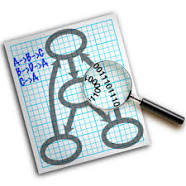
\includegraphics[width=0.2\textwidth]{img/graphviz}
	\end{center}  
\vspace{-20pt}
\vspace{-10pt}  
\end{wrapfigure}
GraphViz (Graph Visualiszation Software) est un ensemble d'outils de visualisation de graphes, créés par les laboratoires de recherche d'AT\&T \citep{graphivz}. Il utilise des fichiers textes suivant le langage $DOT$ pour représenter les données structurées sous forme de graphes. le langage $DOT$ permet  de personnaliser le rendu des graphes par le choix des formes, couleurs et polices de caractères. Ainsi le graphe définie est exporté sous différents formats d'images (FIG, PNG, JPEG, GIF, etc.).

\subsection{Mise en œuvre}
Nous avons développé une application distribuée  implémenter avec le langage de programmation JAVA sur l'IDE IntelliJ. Chaque instance de l'application dispose une base de donnée orienté graphe (Neo4j) pour le stockage de l'espace d'états. Les applications de même réseau sont utilisés pour accomplir une tache de vérification ou de génération de l'espace d'états.

L'application développée pour l'expérimentation de notre approche dispose d’un éditeur graphique pour modéliser le réseau de Pétri du système à analyser (Figure \ref{apppetrinet}). L'outil permet de générer la structure de Kripke distribuée d'un réseau de Pétri modélisé. Il permet  d'exécuter  le model checking sur une structure de Kripke distribuée ainsi que la redistribution de l'espace d'états par l'approche proposée (Figure \ref{mc}).

\begin{figure} [h]
	\centering
	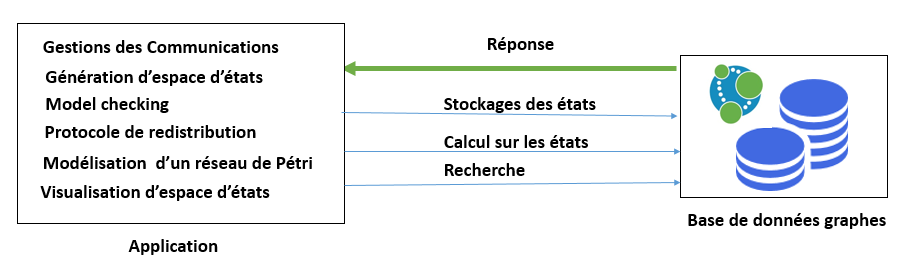
\includegraphics[width=0.7\linewidth]{img/architecture}
	\caption{Architecture de l'application développée}
	\label{fig:architecture}
\end{figure}
\begin{figure} [h]
	\centering
	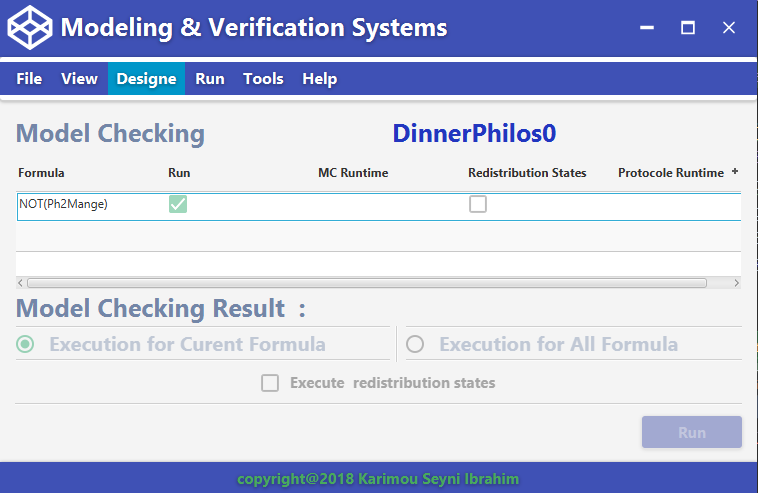
\includegraphics[width=0.7\linewidth]{img/mcapp}
	\caption{Interface d'exécution model checking}
	\label{mc}
\end{figure}
\begin{figure}  
	\centering
	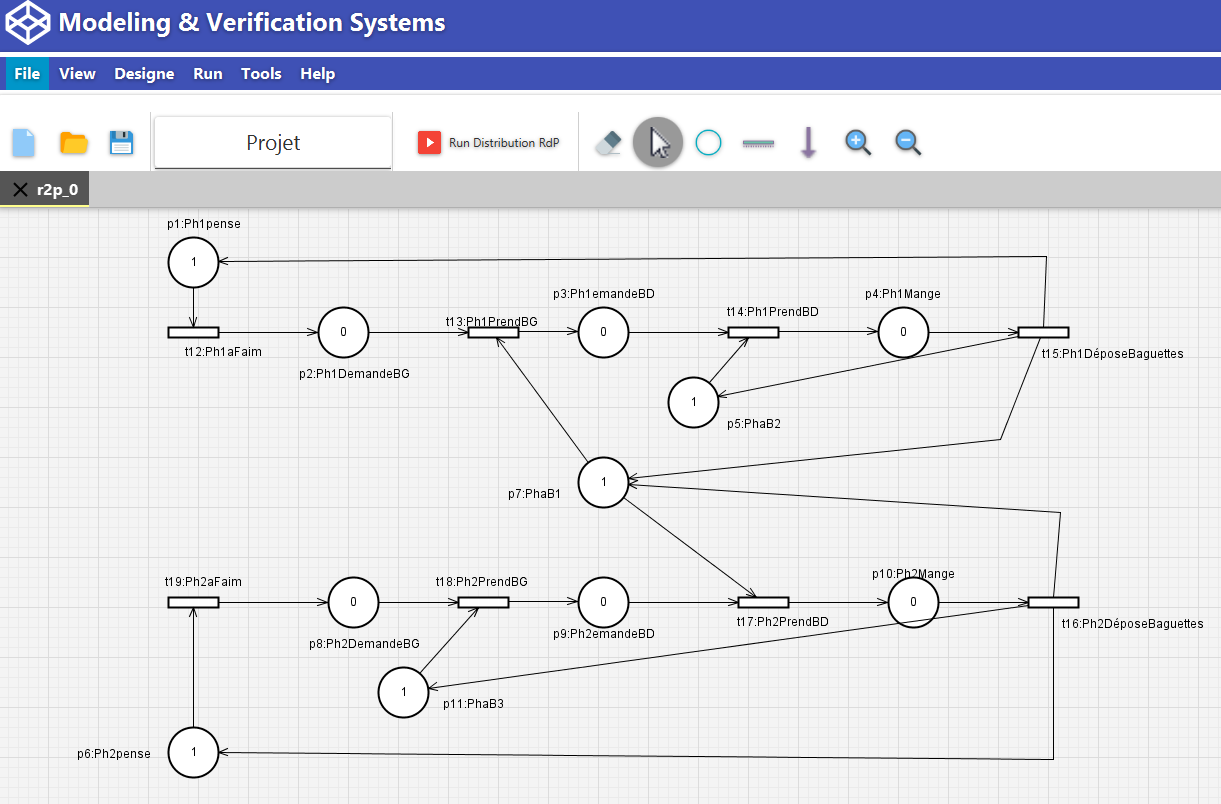
\includegraphics[width=0.7\linewidth]{img/apppetrinet}
	\caption{Éditeur de modélisation d'un réseau de Pétri} \label{apppetrinet}
	\label{fig:apppetrinet}
\end{figure}
\begin{figure} 
	\centering
	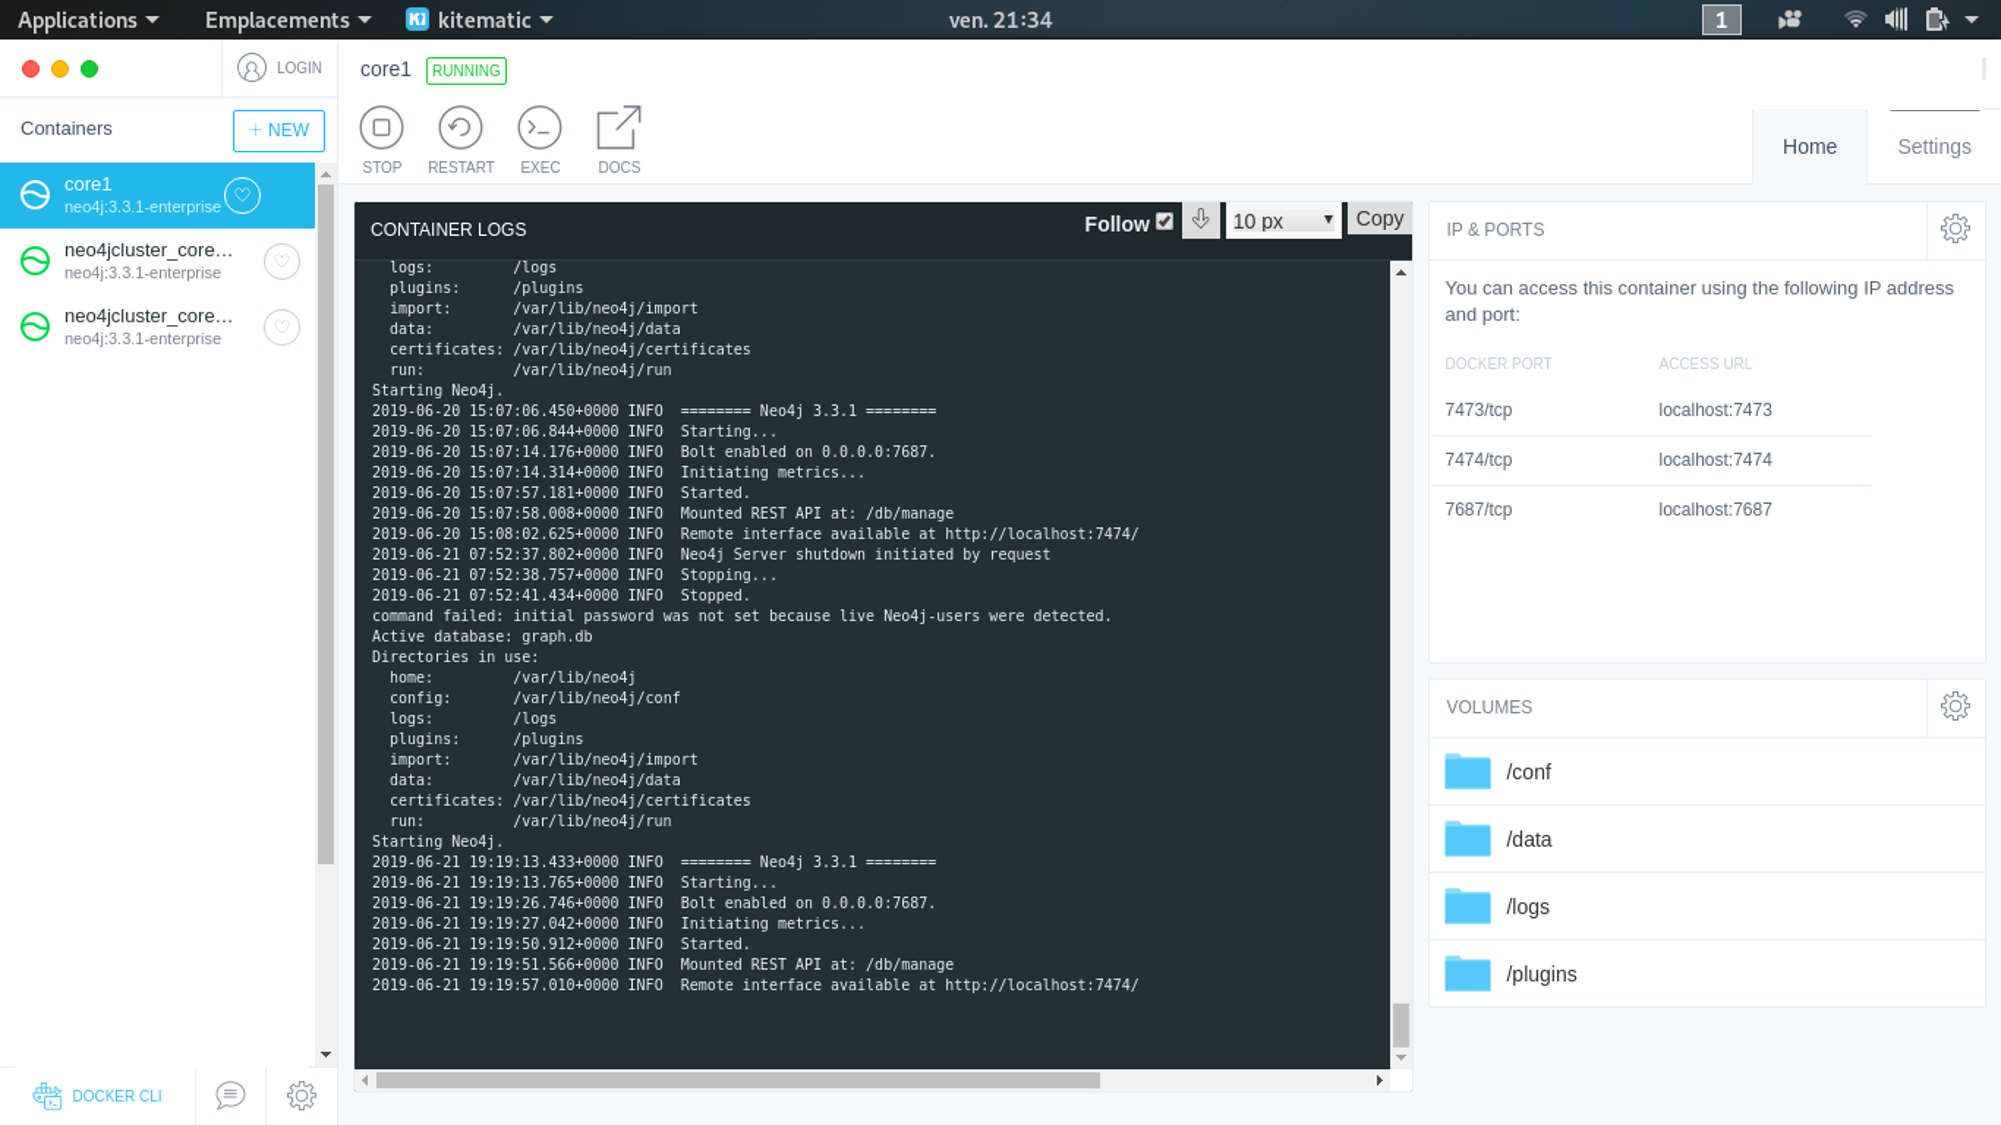
\includegraphics[width=0.7\linewidth]{img/clusterdocker}
	\caption{Virtualisation des Bases de données Neo4j sur Doker}
	\label{fig:clusterdocker}
\end{figure}
\begin{figure} 
	\centering
	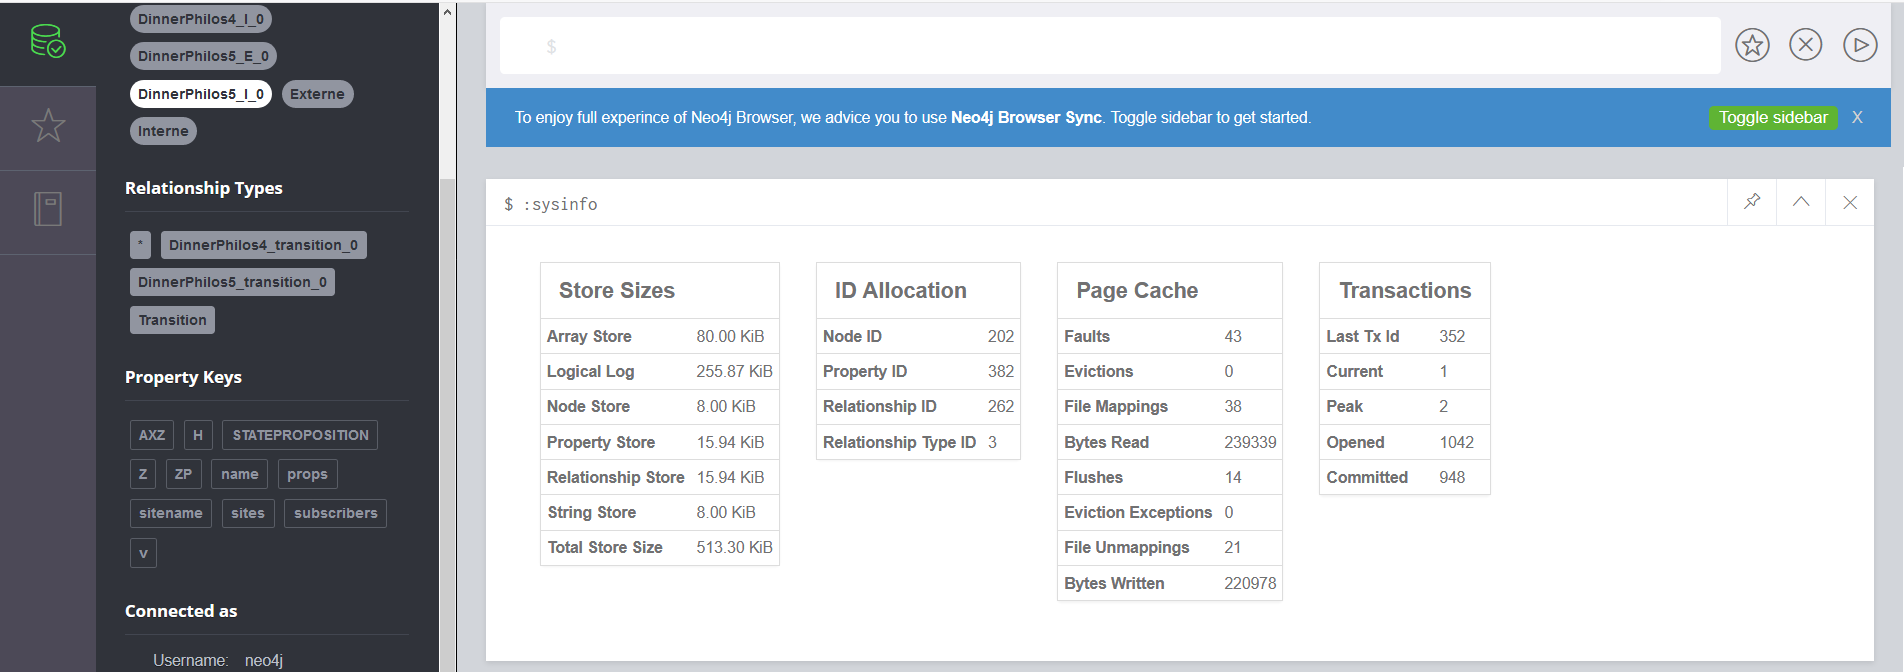
\includegraphics[width=1\linewidth]{img/bddneo4j}
	\caption{Base de données Neo4j} 
\end{figure}
\pagebreak
\subsection{Expérimentation}
Nous avons évalué l’efficacité de la politique de redistribution proposée avec l’approche de distribution basée sur la fonction de hachage MD5 sur le modèle des philosophes. A partir des tableaux \ref{tablea1} et \ref{tableau2}, on constate que l’approche proposée assure une bonne distribution de l'espace d'états pour le model checking tout en maintenant un bon équilibrage de charge, ce qui signifie que toutes les machines du réseau contiennent le nombre d'états qu'il peuvent supporter. En plus du nombre d'états on constate que le temps de la vérification s'améliore de plus en plus, ce qui indique qu’aucune machine n’est surchargée en mémoire et en calcul.

\begin{tableth}
	\centering
	\begin{tabular}{|c|c|c||c||c|c|  }
		\hline
		          Philos            &                Formules                &  Machines   & Temps d'exécution &     Etats Interne      &     Etats Externe      \\ \hline
		\multirow{4}{*}{$2$ Philos} &  \multirow{2}{*}{\tiny NOT(Ph2Mange)}  & Machine $1$ &      $2 s $       &  \multirow{2}{*}{$2$}  &  \multirow{2}{*}{$2$}  \\ \cline{3-4}
		                            &                                        & Machine $2$ &       $2 s$       &                        &                        \\ \cline{2-4}\cline{4-6}
		                            &  \multirow{2}{*}{\tiny NOT(Ph1Mange)}  & Machine $1$ &       $2 s$       &   \multirow{2}{*}{6}   &   \multirow{2}{*}{2}   \\ \cline{3-4}
		                            &                                        & Machine $2$ &      $10 s$       &                        &                        \\ \hline\hline
		\multirow{4}{*}{$3$ Philos} &  \multirow{2}{*}{\tiny NOT(Ph2Mange)}  & Machine $1$ &       $2 s$       & \multirow{2}{*}{$17$ } & \multirow{2}{*}{ $14$} \\ \cline{3-4}
		                            &                                        & Machine $2$ &       $2 s$       &                        &                        \\ \cline{2-4}\cline{4-6}
		                            &  \multirow{2}{*}{\tiny NOT(Ph1Mange)}  & Machine $1$ &      $19 s$       & \multirow{2}{*}{$15$ } & \multirow{2}{*}{$14$ } \\ \cline{3-4}
		                            &                                        & Machine $2$ &      $10 s$       &                        &                        \\ \hline\hline
		\multirow{6}{*}{$4$ Philos} & \multirow{3}{*}{\tiny NOT(Ph2Mange)} & Machine $1$ &      $10 s$       & \multirow{2}{*}{$35$} & \multirow{2}{*}{$53$} \\ \cline{3-4}
		                            &                                        & Machine $2$ &      $19 s$       &                        &                        \\ \cline{3-4}\cline{4-6}
		                            &  \multirow{3}{*}{\tiny NOT(Ph1Mange)}  & Machine $3$ &      $32 s$       &  \multirow{2}{*}{40 }  &  \multirow{2}{*}{49 }  \\ \cline{2-4}
		                            &                                        & Machine $1$ &      $35 s$       &                        &                        \\ \cline{3-4}\cline{4-6}
		                            &                                        & Machine $2$ &      $10 s$       &  \multirow{2}{*}{37 }  &  \multirow{2}{*}{46 }  \\ \cline{3-4}
		                            &                                        & Machine $3$ &      $19 s$       &                        &                        \\ \hline\hline
	\end{tabular}
	\caption{Résultats du model checking sur l'espace d'états distribués avec \textbf{MD5} }\label{tablea1}
\end{tableth}

\begin{tableth}
	\centering
	\begin{tabular}{|c|c|c||c||c|c|c|}
		\hline
		          Philos            &                Formules                &  Machines   & Exécution &     Etats Interne     &     Etats Externe     &       Duplicata       \\ \hline
		\multirow{4}{*}{$2$ Philos} & \multirow{2}{*}{{\tiny NOT(Ph2Mange)}} & Machine $1$ &  $2 s $   & \multirow{2}{*}{$2$}  & \multirow{2}{*}{$2$}  & \multirow{2}{*}{$1$}  \\ \cline{3-4}
		                            &                                        & Machine $2$ &   $2 s$   &                       &                       &                       \\ \cline{2-4}\cline{4-7}
		                            &  \multirow{2}{*}{\tiny NOT(Ph1Mange)}  & Machine $1$ &   $2 s$   & \multirow{2}{*}{$6$}  & \multirow{2}{*}{$2$}  & \multirow{2}{*}{$0$}  \\ \cline{3-4}
		                            &                                        & Machine $2$ &   $2 s$   &                       &                       &                       \\ \hline\hline
		\multirow{4}{*}{$3$ Philos} &  \multirow{2}{*}{\tiny NOT(Ph2Mange)}  & Machine $1$ &   $2 s$   & \multirow{2}{*}{$17$} & \multirow{2}{*}{$14$} & \multirow{2}{*}{$14$} \\ \cline{3-4}
		                            &                                        & Machine $2$ &   $2 s$   &                       &                       &                       \\ \cline{2-4}\cline{4-7}
		                            &  \multirow{2}{*}{\tiny NOT(Ph1Mange)}  & Machine $1$ &  $2 s $   & \multirow{2}{*}{$15$} &  \multirow{2}{*}{14}  &  \multirow{2}{*}{10}  \\ \cline{3-4}
		                            &                                        & Machine $2$ &   $2 s$   &                       &                       &                       \\ \hline\hline
		\multirow{6}{*}{$4$ Philos} &  \multirow{3}{*}{\tiny NOT(Ph2Mange)}  & Machine $1$ &   $2 s$   & \multirow{2}{*}{$35$} & \multirow{2}{*}{$53$} & \multirow{2}{*}{$39$} \\ \cline{3-4}
		                            &                                        & Machine $2$ &   $2 s$   &                       &                       &                       \\ \cline{3-7}
		                            &                                        & Machine $3$ &   $2 s$   & \multirow{2}{*}{$40$} & \multirow{2}{*}{$49$} & \multirow{2}{*}{$36$} \\ \cline{2-4}
		                            &  \multirow{3}{*}{\tiny NOT(Ph1Mange)}  & Machine $1$ &   $2 s$   &                       &                       &                       \\ \cline{3-7}
		                            &                                        & Machine $2$ &   $2 s$   & \multirow{2}{*}{$37$} & \multirow{2}{*}{$46$} & \multirow{2}{*}{$33$} \\ \cline{3-4}
		                            &                                        & Machine $3$ &   $2 s$   &                       &                       &                       \\ \hline\hline
	\end{tabular}
	\caption{Résultats du model checking sur l'espace d'états redistribués avec \textbf{\CDS{}} }\label{tableau2}
\end{tableth}


\def\lasty{}


\begin{tikzpicture}
\draw[thick,<->] (0,8) node[right]{Temps de reponse}--(0,0)--(14,0) node[below]{Formule CTL};

\draw [blue](0,5)--(2,5);
\draw [blue](2,7)--(3,7);
\draw [blue](3,3)--(5,3);
\draw [blue](5,4)--(8,4);
\draw [blue](8,5.5)--(8.5,5.5);
\draw [blue](8.5,2)--(14,2);

\node [below] at (1,0) {$f_1$};

\node [left] at (0,1) {$t_1$};
\node [left] at (0,1.5) {$t_2$};
\node [left] at (0,2) {$t_3$};
\node [left] at (0,3) {$t_4$};
\node [left] at (0,5) {$t_5$};
\node [left] at (0,4) {$t_6$};
\node [left] at (0,7) {$t_8$};
\node [left] at (0,5.5) {$t_7$};

\node [below] at (0,0) {$f_1$};
\node [below] at (1,0) {$f_2$};
\node [below] at (2,0) {$f_3$};
\node [below] at (3,0) {$f_4$};
\node [below] at (4,0) {$f_1$};
\node [below] at (5,0) {$f_2$};
\node [below] at (6,0) {$f_5$};
\node [below] at (7,0) {$f_7$};
\node [below] at (8,0) {$f_2$};
\node [below] at (9,0) {$f_2$};
\node [below] at (10,0) {$f_1$};
\node [below] at (11,0) {$f_2$};
\node [below] at (12,0) {$f_3$};

\draw[red,dashed](2,5)->(2,7);
\draw[red,dashed](5,3)->(5,4);
\draw[green,dashed](3,7)->(3,3);
\draw[red,dashed](8,4)->(8,5.5);
\draw[green,dashed](8.5,5.5)->(8.5,2);


\draw [red, fill=white] (2,5) circle (1.5pt);
\draw [red, fill=white] (5,3) circle (1.5pt);
\draw [red, fill=white] (8,4) circle (1.5pt);


\draw [green] (3,7) circle (1.5pt);
\draw [green] (8.5,5.5) circle (1.5pt);

\end{tikzpicture}
\section{Discussion}

Sur la base des résultats expérimentaux présentés ci-dessus, nous constatons l’efficacité de l’approche proposée pour la distribution de l’espace d'états. En termes d’équilibrage l’approche proposée s’est avérée efficace à cause de sa capacité d’analyser le comportement du système et à extraire les informations pertinentes sur ses états. Ainsi, les résultats ont démontrés que la minimisation des transitions externe n'implique pas toujours la minimisation du temps de calcul. Cependant, Notre approche n'est pas dédiée à réduire le nombre de transitions externes, mais d'analyser les états afin de proposer une distributions adéquats des états tout en garantissant un nombre minimal de communications et un équilibrage de charge entre les machines.
